\section{Dynamics:  Motion Along a Line}

\subsection{The Equilibrium Model}
\begin{definition}[Equilibrium]
    An object is in equilibrium when its net force/acceleration is zero.
\end{definition}
The requirement for equilibrium,
$
    \vec{F}_{net} = \vec{0}
$ and thus
$
    \vec{a}=\vec{0}
$%
, means
\begin{equation}
    (F_{net})_x=\sum_i(F_i)_x=0 \wedge (F_{net})_y=\sum_i(F_i)_y=0
\end{equation}
I.e. the sum of all x-components and y-components must be zero.

\subsection{Using Newton's Second Law} The essence of Newtonian
mechanics can be expressed in two steps
\begin{enumerate}
    \item
        The forces acting on an object can determine its acceleration
        $
            \vec{a}=\vec{F}_{net}/m
        $%
        .
    \item
        The object's trajectory can be determined by using
        $
            \vec{a}
        $ in the kinematic equations.
\end{enumerate}
\begin{Exercise}[title={Speed of a towed car}, label={dynamics.2.1},
    origin={Knight}]
    A 1500 kg car is pulled by a tow truck.  The tension in the tow rope
    is 2500 N, and a 200 N friction force opposes the motion.  If the
    car starts from rest, what is its speed after 5.0 seconds?
    \begin{figure}[!htbp]
        \centering
        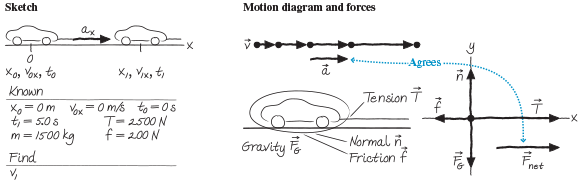
\includegraphics[width=0.6\textwidth]{../figures/car-towed-pictoral-representation.png}
        \caption{Model of car being towed%
        \label{dynamics.2.2}}
    \end{figure}
\end{Exercise}
\begin{Answer}[ref={dynamics.2.1}]

    Looking at Figure~%
    \ref{dynamics.2.2} we create the table
    \begin{equation}
        \label{dynamics.2.1-Answer.1}
        \begin{array}{|l|l|l|}
            \hline
            \text{Force} & \text{x-component} & \text{y-component} \\
            \hline
            \vec{n} & 0 & +n \\
            \hline
            \vec{T} & +2500 & 0 \\
            \hline
            \vec{f} & -200 & 0 \\
            \hline
            \vec{F}_G & 0 & F_G \\
            \hline
            \vec{a} & a & 0 \\
            \hline
        \end{array}
    \end{equation}
    \begin{remark}
        As acceleration
        $
            \vec{a}
        $ is just the net force
        $
            \vec{F}_{net}
        $ scaled by the inverse mass
        $
            1/m
        $%
        , it points in the same direction as
        $
            \vec{F}_{net}
        $%
.        Thus, the y-component of
        $
            \vec{a}
        $ is 0.
    \end{remark}

    Using Newton's second law:
    \begin{equation}
        \begin{split}
            (F_{net})_x=\sum F_x=T_x+f_x+n_x+(F_G)_x=ma_x \\
            (F_{net})_y=\sum F_y=T_y+f_y+n_y+(F_G)_y=ma_y
        \end{split}
    \end{equation}
    we find
    \begin{align}
        a_x &= \frac{1}{m}(T+f) \\
        &= \frac{1}{\qty{1500}{\kilo\gram}}(\qty{2500}{\newton}-\qty{200}
        {\newton}) = \qty{1.53}{\metre\per\square\second} \\
        a_y &= \frac{1}{m}(n-(F_G))
    \end{align}
    \begin{remark}
        Since the y-component of
        $
            \vec{a}
        $ is zero, we conclude that
        $
            n=F_G
        $
    \end{remark}

    Because
    $
        a_x
    $ is constant, we can find the speed the truck moves after five
    seconds from rest:
    \begin{align}
        v_{fx}&=v_{ix}+a_x\Delta t \\
        &= 0+(\qty{1.53}{\metre\per\square\second})(\qty{5.0}{\second})=\qty
        {7.7}{\metre\per\second}
    \end{align}
    Thus, the speed of the truck after being towed for five seconds is
    $
        \qty{7.7}{\metre\per\second}
    $%
    .
\end{Answer}

If all forces are constants over time, like in Example~%
\ref{dynamics.2.1}, then the acceleration will be constant.  If the
acceleration is constant, we can deploy the uniform acceleration model
of kinematics.

\subsection{Mass}

\begin{definition}[Mass]
    A scalar quantity that describes an object's inertia
\end{definition}
Mass tells us something about an object regardless of where it is, what
it's doing, or what forces are being applied to it.

\subsection{Gravity}

\begin{definition}[Gravity]
    An attractive, long-range force between any two objects.
\end{definition}

\begin{theorem}[Newton's Law of Gravity]
    \label{theo:newtons-law-of-gravity} For any two objects with masses
    $
        m_1
    $ and
    $
        m_2
    $ seperated by distance
    $
        r
    $%
.    Each object pulls on each other with a force of
    \begin{equation}
        \frac{Gm_1m_2}{r^2}
    \end{equation}
    where
    $
        G=\qty{6.67e-11}{\newton\square\metre\per\square\kilogram}
    $%
    , called the \emph{gravitational constant}, is one of the basic
    constants of nature.
    \begin{remark}
        Gravity is not a constant force, and gets weaker as the distance
        between the objects increases.
    \end{remark}
\end{theorem}

An example of Theroem~%
\ref{theo:newtons-law-of-gravity} is given by Figure~%
\ref{fig:newtons-law-of-gravity}.
\begin{figure}
    \centering
    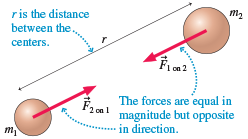
\includegraphics[width=0.4\textwidth]{../figures/newtons-law-of-gravity.png}
    \caption{Newton's law of gravity}%
    \label{fig:newtons-law-of-gravity}
\end{figure}

\begin{figure}
    \centering
    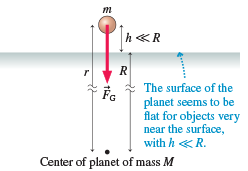
\includegraphics[width=0.4\textwidth]{../figures/flat-earth-approx.png}
    \caption{Gravity near surface of plant}%
    \label{fig:flat-earth-approx}
\end{figure}

Gravitational force is negligible if not from something like a planet.
For an object moving near the surface of a planet, we can make a \textbf
{flat-earth approximation}, shown in Figure~%
\ref{fig:flat-earth-approx}.  That is, for an object whose height above
the surface is very small in comparison with the size of the planet,
then the curvature of the surface is not noticable.  Thus,
$
    r
$ is approximately the planet's radius
$
    R
$%
.  Consequently, a good approximation of the gravitational force of the
planet on mass
$
    M
$ is
\begin{equation}
    \vec{F}_G=\vec{F}_{planet~on~m}=\left(\frac{GM}{R^2},\mathrm{~straight~down}\right)=\left
    (mg,\text{~straight~down}\right)%
    \label{=:flat-earth-approx}
\end{equation}
The magnitude of gravitational force is
$
    F_G = mg
$ where
$
    g
$ is
\begin{equation}
    g=\frac{GM}{R^2}
\end{equation}

Since force is defined as
$
    F=ma
$%
, we see in Equation~%
\ref{=:flat-earth-approx}
$
    g
$ is the acceleration that
$
    F_G
$ causes on mass
$
    M
$%
.

\subsection{Static Friction}

\begin{definition}[Static Friction]
    The force that keeps an object from slipping.
\end{definition}

\begin{figure}
    \centering
    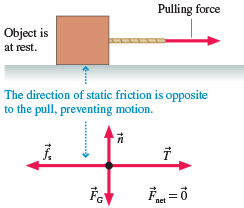
\includegraphics[width=0.4\textwidth]{../figures/static-friction.png}
    \caption{Static friction keeps an object from slipping}%
    \label{fig:static-friction}
\end{figure}

\begin{figure}
    \centering
    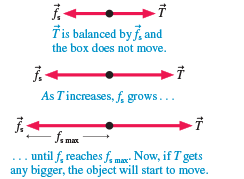
\includegraphics[width=0.4\textwidth]{../figures/static-friction-response.png}
    \caption{Static friction responding to an applied force}%
    \label{fig:static-friction-response}
\end{figure}
Figure~%
\ref{fig:static-friction} shows a rope pulling a box that, due to static
friction, is not moving.  The box is in equilibrium so the static
friction must be exactly equal to the tension force
\begin{equation}
    f_s=T
\end{equation}
The size of static friction depends on how hard you push or pull.
Static friction acts in \emph{response} to am applied force.  This idea
is shown by Figure~%
\ref{fig:static-friction-response}.

If you pull hard enough, the object slips and starts to move.  I.e., the
static friction has a \emph{maximum} magnitude
$
    f_{s~\mathrm{max}}
$ and starts slipping when
$
    f_s=f_{s\mathrm{~max}}
$%
.

Experiements with friction show that
$
    f_{s~\mathrm{max}}
$ is proportional to the magnitude of the normal force.  That is,
\begin{equation}
    f_{s~\mathrm{max}}=\mu_sn
\end{equation}
where the proportionality constant
$
    \mu_s
$ is called the \textbf{coefficient of static friction}.  The
coefficient is a dimensionless constant that depends on the material the
object is on.

\subsection{Kinetic Friction}

Once the box starts to slide, the static force is replaced by a kinetic
friction force
$
    \vec{f}_k
$%
.  Experiments show that unlike static friction, kinetic friction's
magnitude is constant.  Furthermore, the size of the magnitude of
kinetic friction force is less than the maximum static friction and
proportional to the magnitude of the normal force:
\begin{equation}
    f_k=\mu_kn
\end{equation}
where
$
    \mu_k
$ is called the \textbf{coefficient of kinetic friction}.
